\documentclass[11pt]{article}
\usepackage[margin=1in]{geometry}
\usepackage{graphicx}
\usepackage{hyperref}
\usepackage[font=small,labelfont=bf]{caption}

\title{Figure Compilation — Runaround Smooth}
\author{Auto-generated from figure\_registry\_concise.txt}
\date{\today}

\begin{document}
\maketitle
\listoffigures
\clearpage

\begin{figure}[htbp]
  \centering
  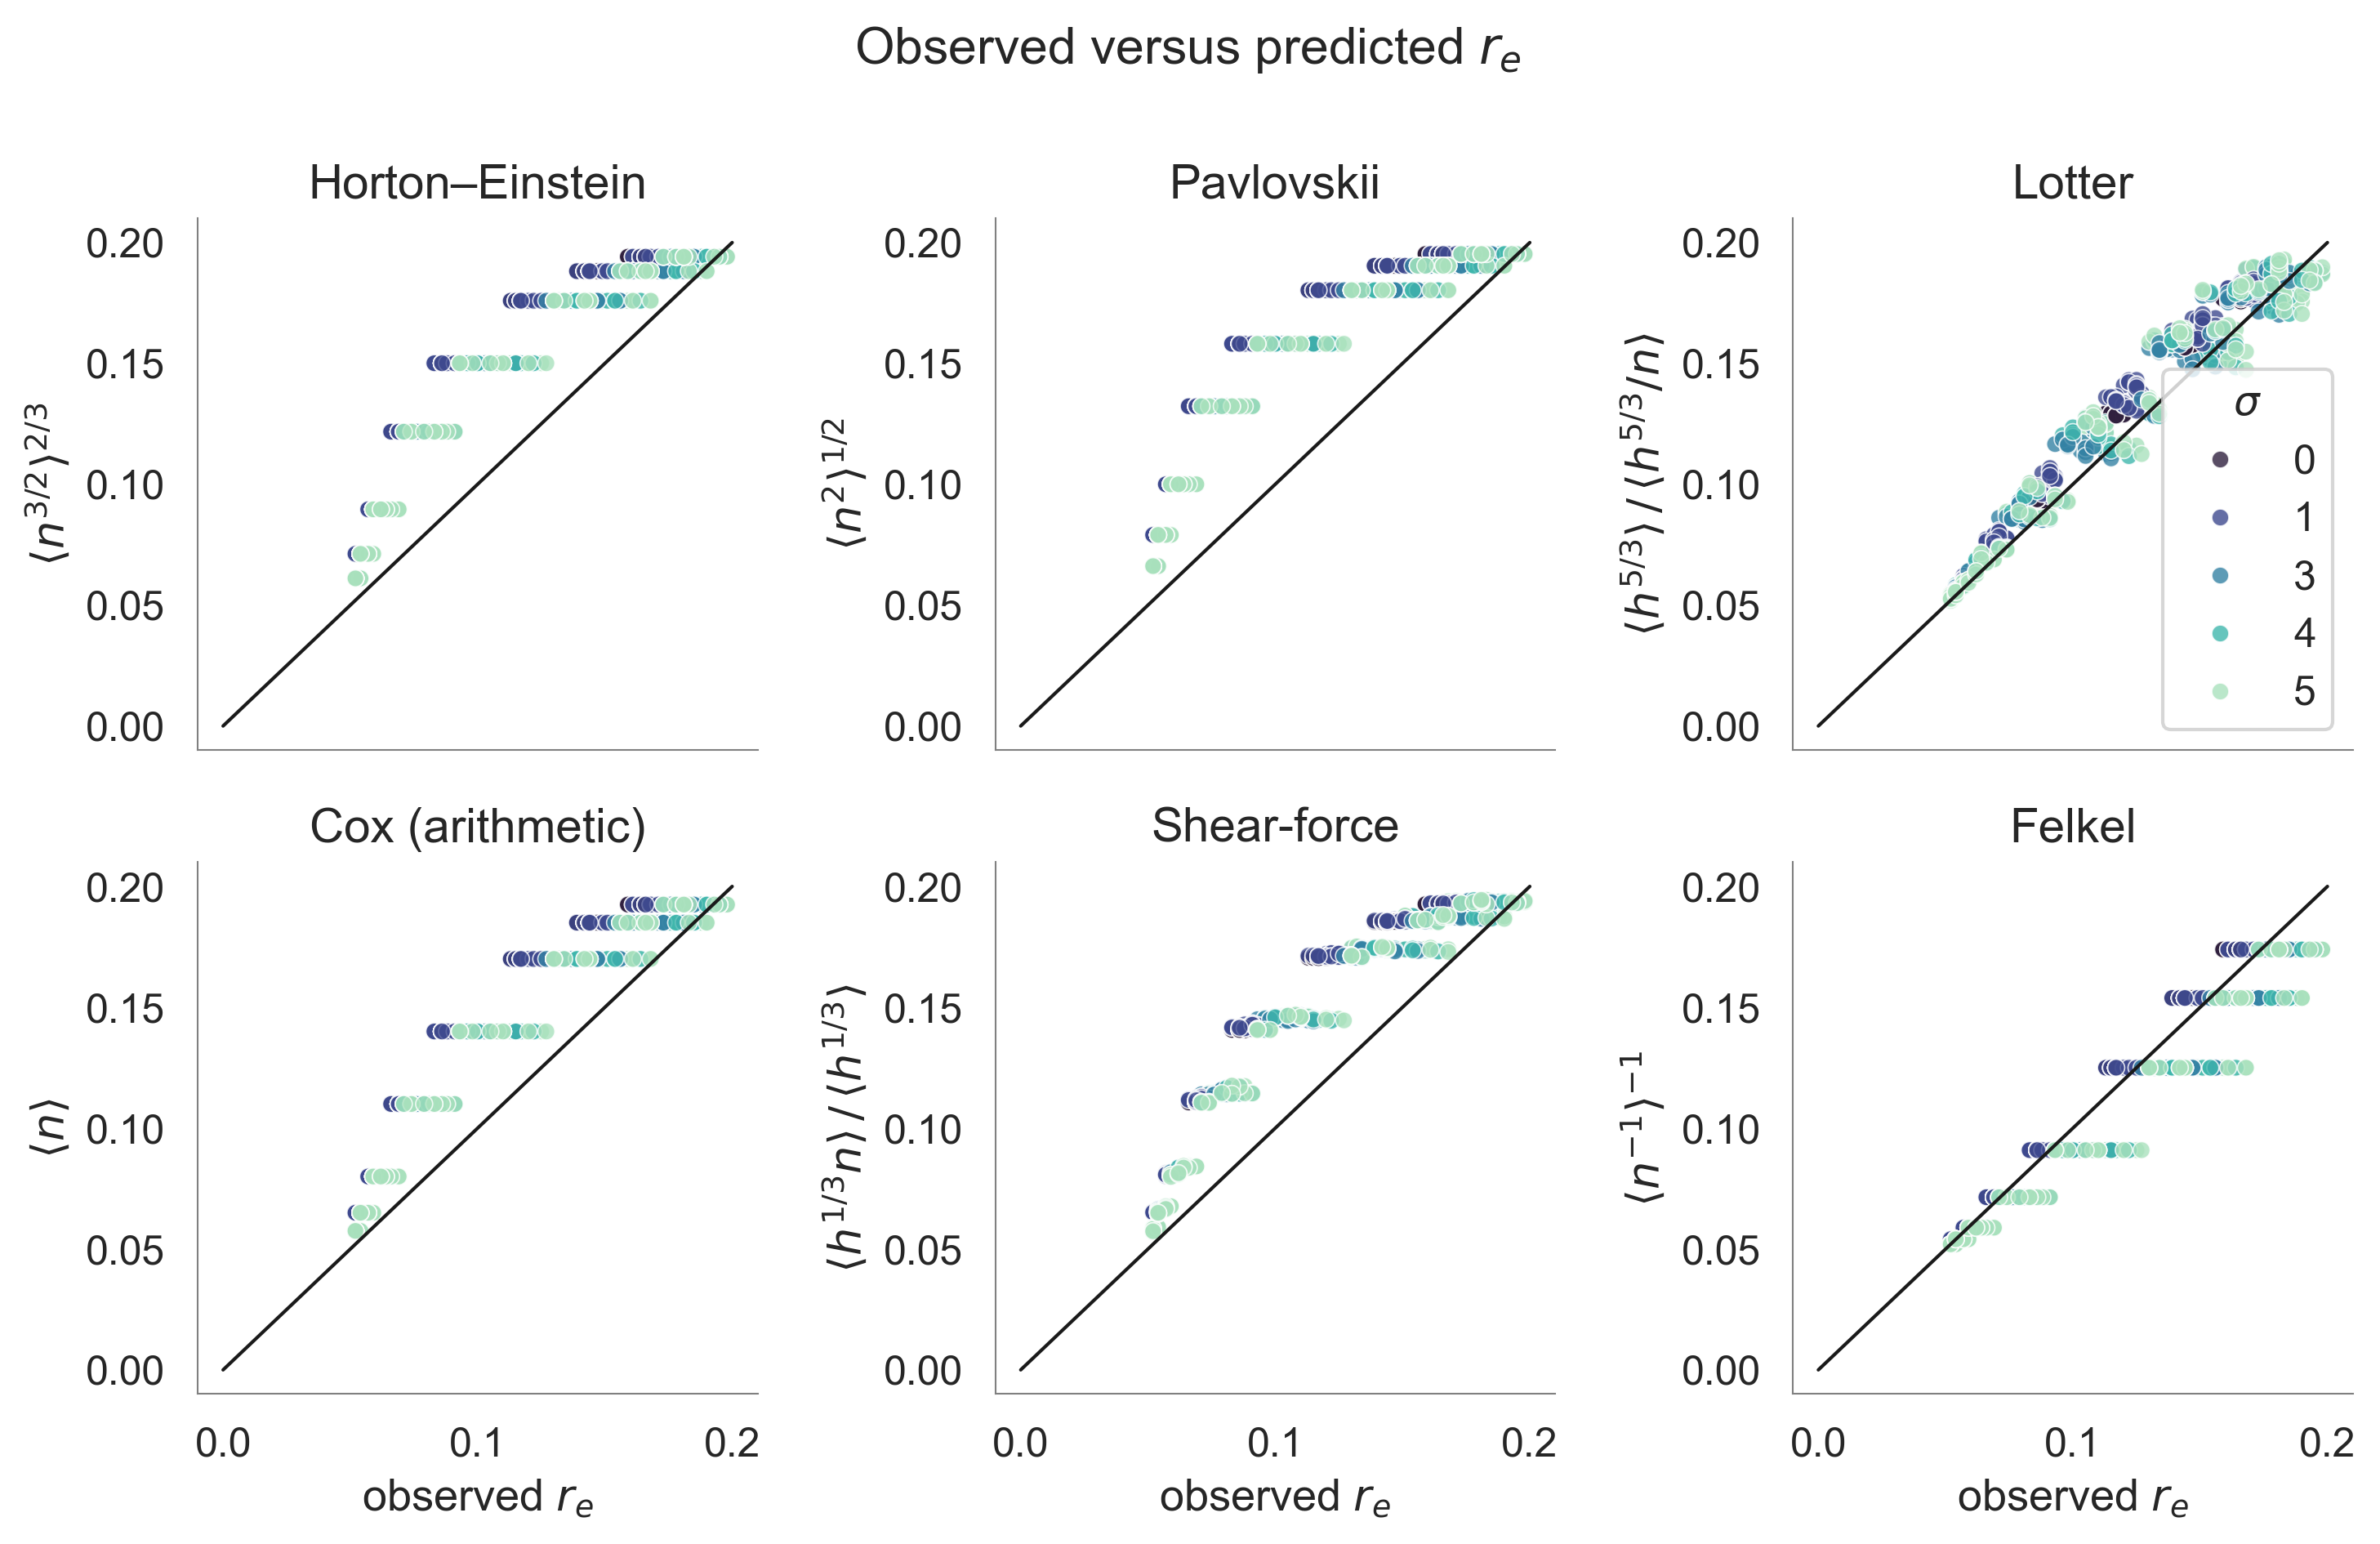
\includegraphics[width=\textwidth]{../figures/runaround_smooth/fig4_obs_vs_pred_re_6panel.png}
  \caption{2×3 observed vs predicted r\_e for six composite-roughness expressions, coloured by sigma. Felkel and Horton-Einstein track the 1:1 line best; Cox is insensitive.}
  \label{fig:fig4}
\end{figure}


\begin{figure}[htbp]
  \centering
  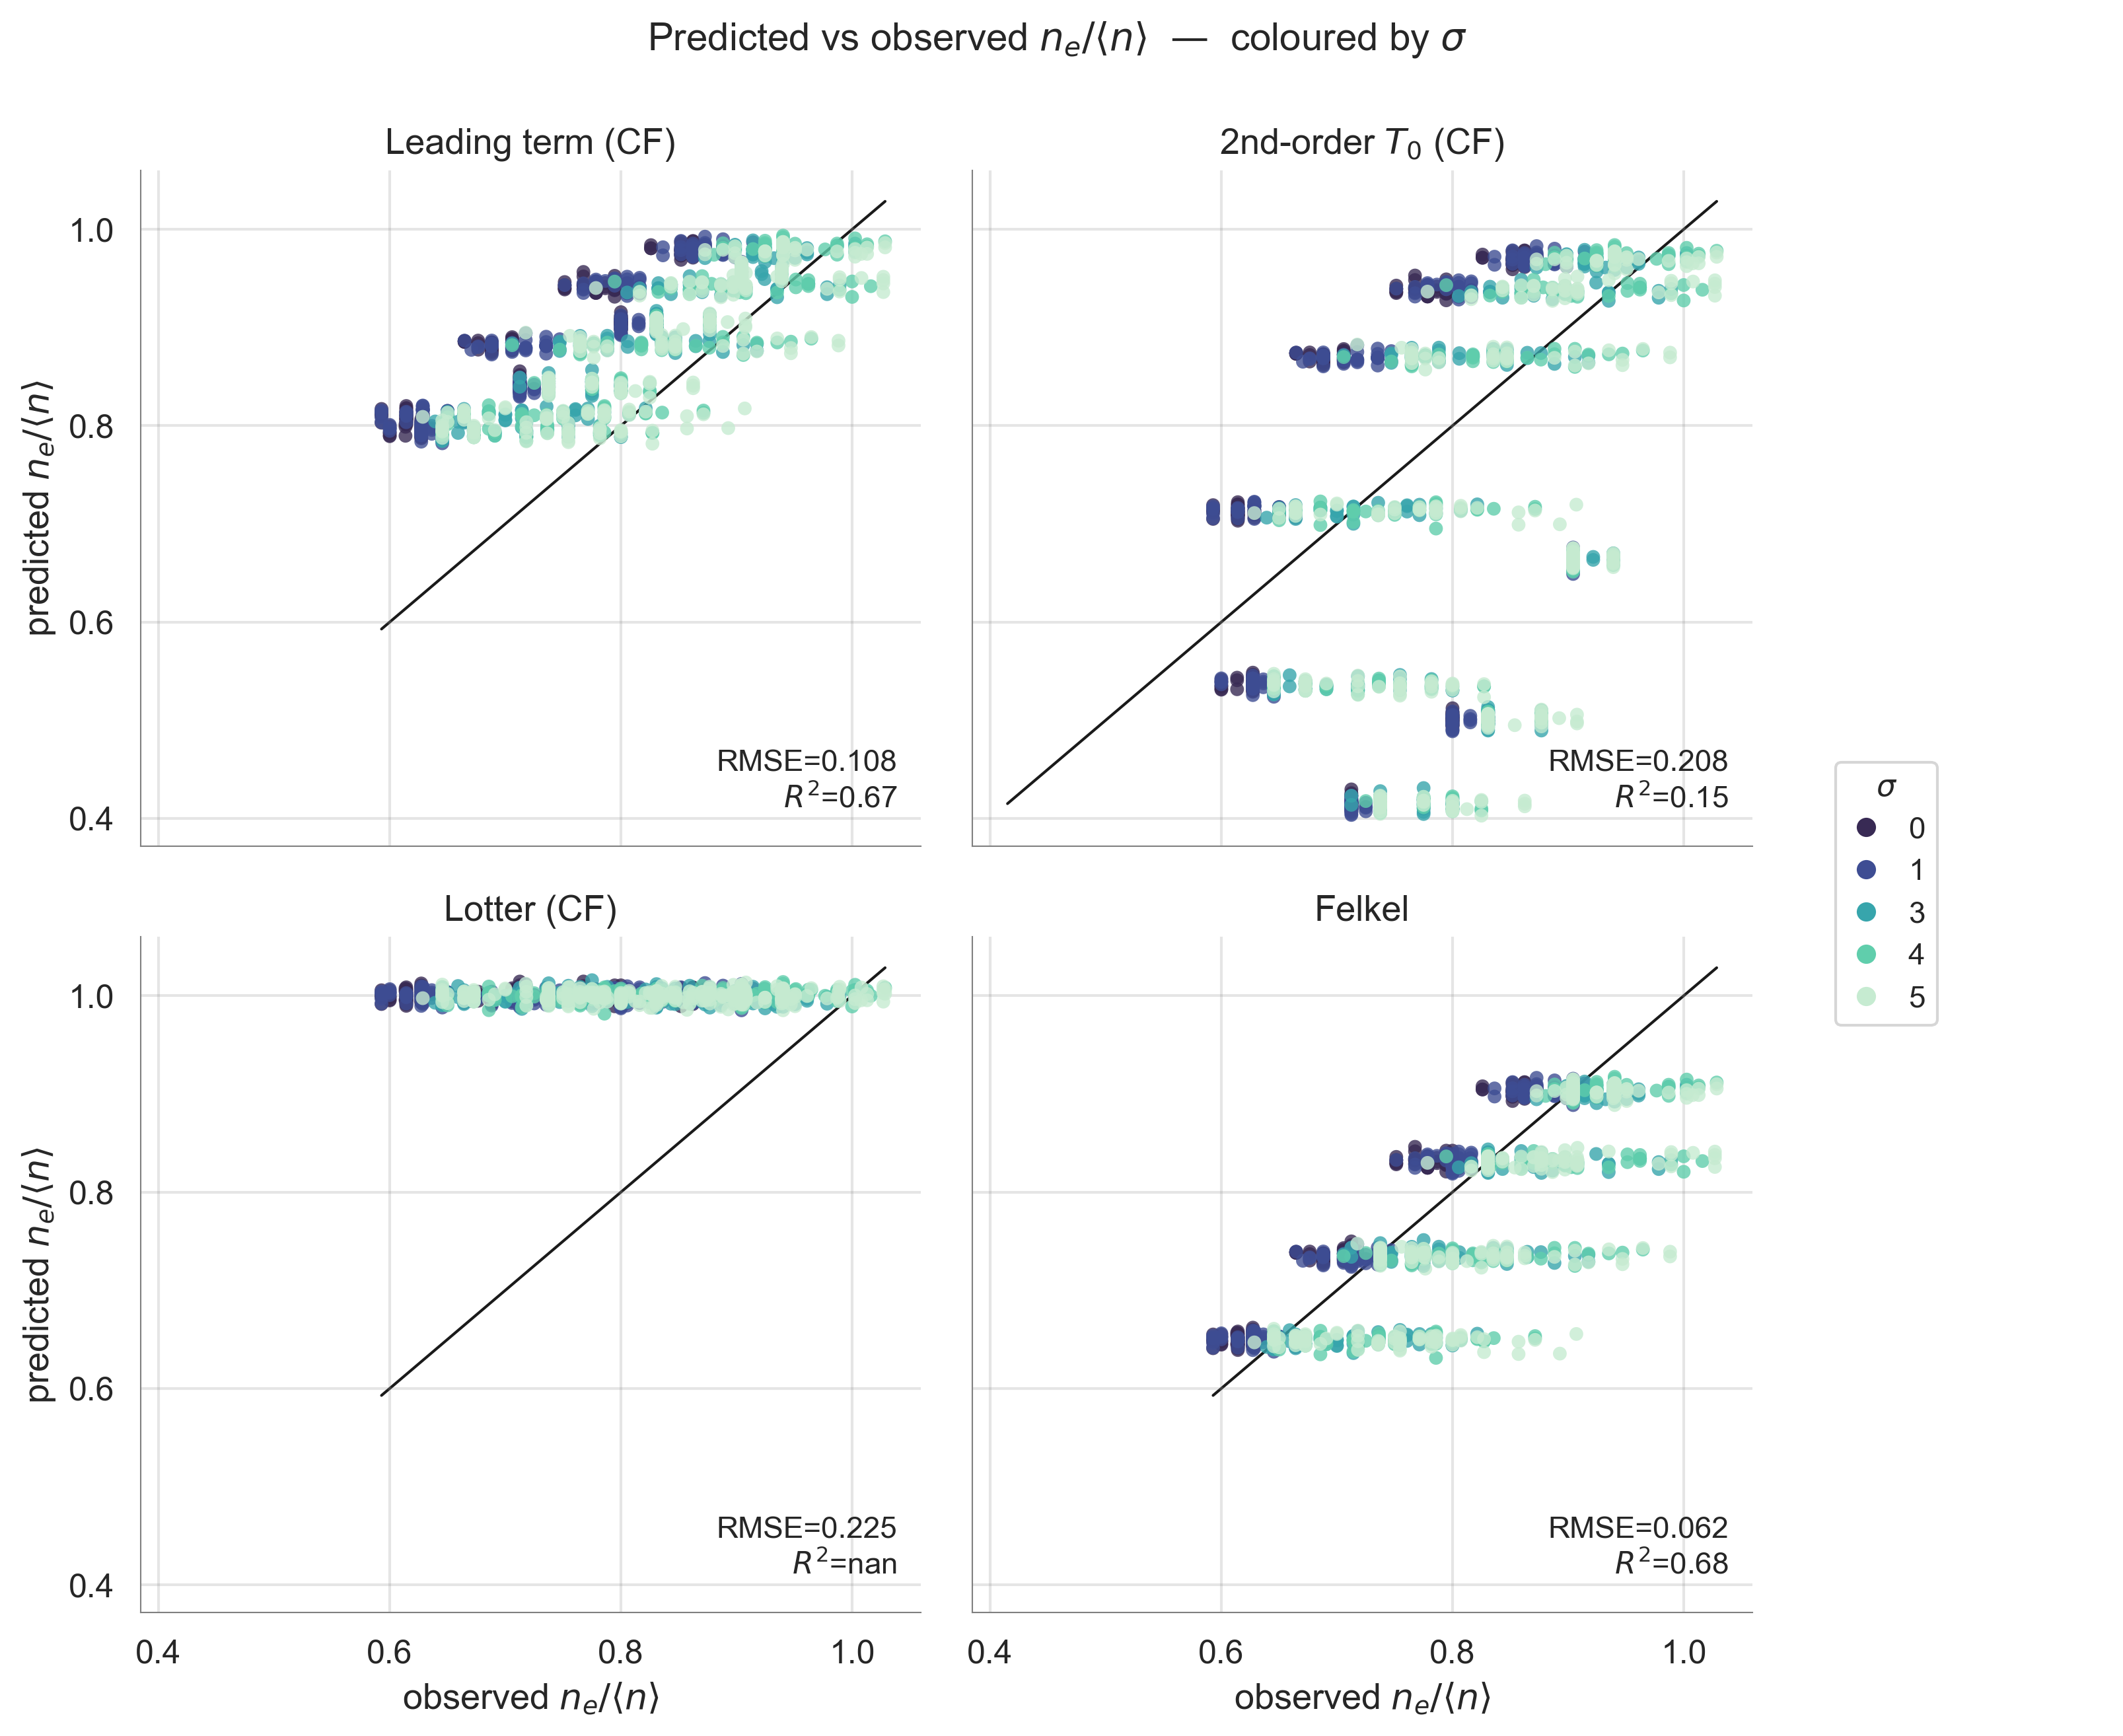
\includegraphics[width=\textwidth]{../figures/runaround_smooth/fig5_pred_vs_obs_CF.png}
  \caption{2×2 predicted vs observed n\_e/<n> for four CF methods, coloured by sigma. Leading-term CF captures most variance (R²$\approx$0.67); Lotter predicts a constant and cannot distinguish cases.}
  \label{fig:fig5}
\end{figure}

\end{document}
